
隊列是一個非常簡單的數據結構,可以從兩端訪問的數組:數據添加到數組的隊尾,在隊頭刪除數據。實現時,隊列和堆棧還是有一些區別和相似的,接下來我們會經常將隊列和堆棧進行對比。

就像堆棧一樣,STL也有隊列容器\texttt{std::queue},當涉及到併發性時,也有相同的問題:刪除元素的接口不是事務性的,需要三個獨立的成員函數共同完成。如果使用帶有鎖的\texttt{std::queue}創建一個線程安全的隊列,就必須像堆棧那樣對其進行包裝:

\hspace*{\fill} \\ %插入空行
\noindent
\textbf{03\_queue.C}
\begin{lstlisting}[style=styleCXX]
template <typename T> class mt_queue {
	std::queue<T> s_;
	mutable spinlock l_;
	public:
	void push(const T& v) {
		std::lock_guard g(l_);
		s_.push(v);
	}
	std::optional<T> pop() {
		std::lock_guard g(l_);
		if (s_.empty()) {
			return std::optional<T>(std::nullopt);
		} else {
			std::optional<T> res(std::move(s_.front()));
			s_.pop();
			return res;
		}
	}
};
\end{lstlisting}

這裡使用自旋鎖(比互斥鎖快)。\texttt{front()}的實現方式與\texttt{pop()}相似,只是不需要刪除頭部元素。基準測試會測量“一個元素推入隊列,並將其彈出”所花費的時間。使用上一節中做測試的x86機器,可以得到以下的結果:

%\hspace*{\fill} \\ %插入空行
\begin{center}
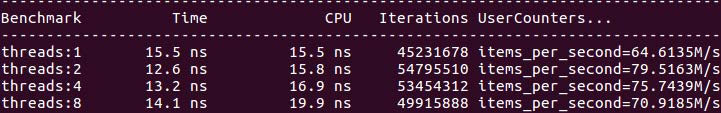
\includegraphics[width=0.9\textwidth]{content/2/chapter7/images/17.jpg}\\
圖7.17 - 由自旋鎖保護的\texttt{std::queue}性能
\end{center}

為了進行比較,在相同的硬件上,沒有鎖的\texttt{std::queue}每秒可以發送280M個元素(一個item表示\texttt{push}和\texttt{pop},所以這裡測試的是每秒可以通過隊列吞吐多少個元素)。其結果與堆棧的情況非常相似,為了比鎖保護的版本更好,必須嘗試一下無鎖實現。

\subsubsubsection{7.4.1\hspace{0.2cm}無鎖隊列}

開始設計無鎖隊列之前,要對每個事務進行詳細的分析,就像對堆棧那樣。同樣,假設隊列建立在一個數組或類似數組的容器上(這裡推遲討論關於數組存滿時會發生的問題)。將元素推入隊列看起來就像堆棧一樣:

%\hspace*{\fill} \\ %插入空行
\begin{center}
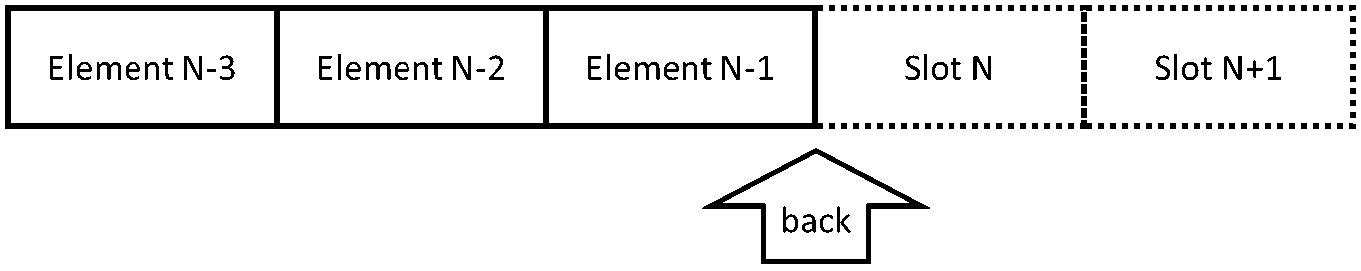
\includegraphics[width=0.9\textwidth]{content/2/chapter7/images/18.jpg}\\
圖7.18 - 在隊列尾部添加元素(生產者視角)
\end{center}

這裡需要數組中第一個空槽的下標。然而,從隊列中刪除元素與在堆棧上的相同操作不同。可以在圖7.19中看到(與圖7.9比較):

%\hspace*{\fill} \\ %插入空行
\begin{center}
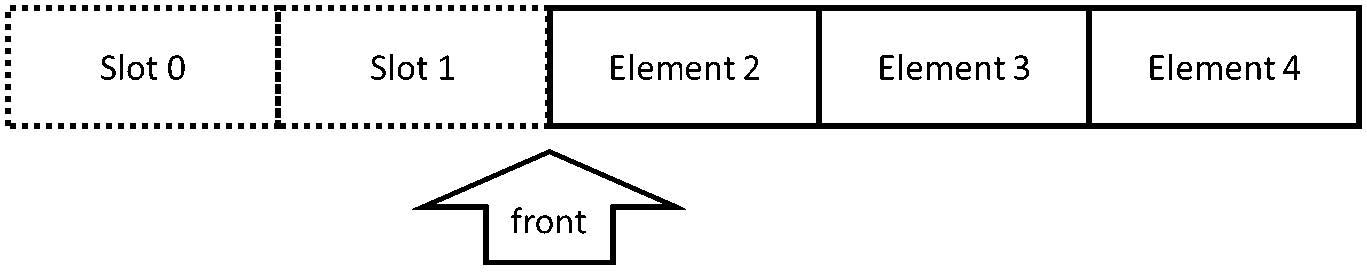
\includegraphics[width=0.9\textwidth]{content/2/chapter7/images/19.jpg}\\
圖7.19 - 在隊頭部移除元素(消費者視角)
\end{center}

元素從隊列的頭部刪除,因此需要尚未刪除的第一個元素的索引(隊列當前的頭)。

現在來看看隊列和堆棧之間的區別。堆棧中,生產者和消費者都在同一個位置上操作:堆棧的頂部。若生產者開始在堆棧頂部構造新元素,消費者就必須等待其完成。\texttt{pop}操作不能返回最後一個構造的元素,而不會在數組中留下一個空洞,而且在構造完成之前,不能返回正在構造的元素。

對於隊列來說,情況就不同了。只要隊列不是空的,生產者和消費者就根本不會交互。\texttt{push}操作不需要知道頭部的索引是什麼,而\texttt{pop}操作不關心隊尾的索引。生產者和消費者不會對同一內存位置的訪問進行競爭。

當遇到這樣的情況,即有幾種不同的方式來訪問數據結構,並且它們(大多數)不相互交互。建議首先考慮將這些角色分配給不同線程的場景,進一步簡化使用每一種線程的方式。我們的例子中,其意味著一個生產者線程和一個消費者線程。 

因為只有生產者需要訪問返回索引,而且只有一個生產者線程,不需要為這個索引使用原子整數。類似地,索引只是普通整數。在隊列變為空時,兩個線程才會交互。為此,需要一個原子變量,表示隊列的大小。生產者在第一個空槽中構造新元素,並向前推進返回索引(可以以任何順序,因為只有一個生產者線程)。然後,增加隊列的大小,以反映隊列現有的元素數量。 

消費者必須按相反的順序操作。檢查隊列大小,確保隊列不為空。然後消費者可以從隊列中獲取第一個元素,並推進隊列頭部的索引。當然,不能保證在檢查和訪問頭部元素時,隊列大小不會改變。但這也不會引起任何問題。因為,只有一個消費者線程,而生產者線程只能增加隊列大小。

在探索堆棧的過程中,沒討論向數組添加更多內存的問題,並假設已知堆棧的最大容量,並且不會超過(如果超過了該容量,也可以使\texttt{push}操作失敗)。對於隊列來說,同樣的假設就不夠了。隨著元素的添加和從隊列中刪除,前後的索引都會移動,並最終到達數組的末尾。當然,數組的第一個元素未使用,所以最簡單的解決方案是將數組視為循環緩衝區,並對數組下標使用取模運算:

\hspace*{\fill} \\ %插入空行
\noindent
\textbf{03a\_atomic\_pc\_queue.C}
\begin{lstlisting}[style=styleCXX]
template <typename T> class pc_queue {
public:
	explicit pc_queue(size_t capacity) : 
	capacity_(capacity),
	data_(static_cast<T*>(::malloc(sizeof(T)*capacity_))) {}
	~pc_queue() { ::free(data_); }
	bool push(const T& v) {
		if (size_.load(std::memory_order_relaxed) >= capacity_)
		return false;
		new (data_ + (back_ % capacity_)) T(v);
		++back_;
		size_.fetch_add(1, std::memory_order_release);
		return true;
	}
	std::optional<T> pop() {
		if (size_.load(std::memory_order_acquire) == 0) {
			return std::optional<T>(std::nullopt);
		} else {
			std::optional<T> res(
			std::move(data_[front_ % capacity_]));
			data_[front_ % capacity_].~T();
			++front_;
			size_.fetch_sub(1, std::memory_order_relaxed);
			return res;
		}
	}
private:
	const size_t capacity_;
	T* const data_;
	size_t front_ = 0;
	size_t back_ = 0;
	std::atomic<size_t> size_;
};
\end{lstlisting}

隊列需要一個特殊的基準測試,因為在設計上受了一些限制:一個生產者線程和一個消費者線程:

\hspace*{\fill} \\ %插入空行
\noindent
\textbf{03a\_atomic\_pc\_queue.C}
\begin{lstlisting}[style=styleCXX]
pc_queue<size_t> q(1UL<<20);
void BM_queue_prod_cons(benchmark::State& state) {
	const bool producer = state.thread_index & 1;
	const size_t N = state.range(0);
	for (auto _ : state) {
		if (producer) {
			for (size_t i = 0; i < N; ++i) q.push(i);
		} else {
			for (size_t i = 0; i < N; ++i) 
			benchmark::DoNotOptimize(q.pop());
		}
	}
	state.SetItemsProcessed(state.iterations()*N);
}
BENCHMARK(BM_queue_prod_cons)->Arg(1)->Threads(2)
->UseRealTime();
BENCHMARK_MAIN();
\end{lstlisting}

為了進行比較,應該在相同的條件下對鎖保護的隊列進行基準測試(鎖的性能通常對線程競爭非常敏感)。同一臺x86機器上,兩個隊列的吞吐量大致相同,為每秒100M個整數元素。在ARM處理器上,鎖相對來說更耗時,我們的隊列也不例外:

%\hspace*{\fill} \\ %插入空行
\begin{center}
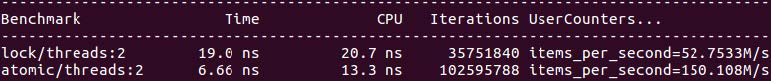
\includegraphics[width=0.9\textwidth]{content/2/chapter7/images/20.jpg}\\
圖7.20 - ARM上基於鎖的整數隊列與無鎖整數隊列的性能對比
\end{center}

即使是在x86上,分析也不完整。前一節中,若堆棧元素很大,那麼複製所需的時間要長於線程同步(鎖定或原子操作)。因為大多數時候,一個線程仍然需要等待另一個線程完成複製,所以不能充分利用使用這個堆棧,從而提出了替代方案:指針堆棧,將實際數據存儲在其他地方。缺點是需要另一個線程安全的容器,來存儲這些數據(程序需要將其存儲在某個地方)。對於隊列來說,這仍然是可行的建議,但現在有了另一個選擇。隊列中的生產者和消費者線程不會互相等待,它們的交互在檢查大小後結束。如果數據元素很大,那麼無鎖隊列就有優勢,因為兩個線程可以同時複製數據,並且比起線程競爭的時間要短得多。要進行這樣的基準測試,只需要創建一個大型對象隊列,比如一個包含大型數組的結構體。即使是在x86硬件上,也如預期的一樣,無鎖隊列執行的更快:

%\hspace*{\fill} \\ %插入空行
\begin{center}
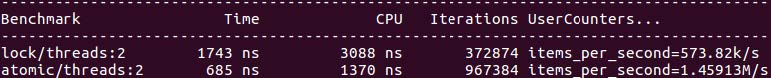
\includegraphics[width=0.9\textwidth]{content/2/chapter7/images/21.jpg}\\
圖7.21 - x86上基於鎖的隊列與無鎖隊列的性能對比
\end{center}

即使有強加的限制,這也是非常有用的數據結構。當已知隊列元素數量的上限時,這個隊列可以用於在生產者和消費者線程之間傳輸數據,或者處理生產者在推送數據前的情況(等待)。隊列非常高效,更重要的是它具有非常低的、可預測的延遲:隊列本身沒有鎖,也沒有等待。線程間不需要互相等待,除非隊列已滿。如果消費者必須對隊列中獲取的數據元素進行處理,並且開始的消費能力小於隊列增加的速度,這樣隊列很快會填滿。這時,常見的方法是讓生產者處理不能入隊的元素。這將在生產者線程產生延遲,直到消費者能夠趕上生產的速率(因為會無序地處理數據,這種方法並不適用於每個程序,但通常非常高效)。

對於許多生產者或消費者線程的情況,隊列的泛化將使實現更加複雜。即使使前後端索引原子化,基於原子的無等待算法也無法工作。如果多個消費者線程讀取一個非零的值,這不再足以讓其他線程繼續。對於多個使用者,當一個線程檢查發現非零時,大小可以減少,並變為零(在第一個線程測試大小之後,在嘗試訪問隊列前端之前,其他線程彈出了所有元素)。

通用的解決方案是使用與堆棧相同的技術,將\texttt{front}和\texttt{back}索引打包到一個64位原子類型中,並使用比較-交換以原子方式訪問。其實現類似於堆棧的實現,理解了上一節中的代碼的讀者可以來實現這個隊列了。在文獻中還可以找到其他無鎖隊列解決方案,本章將提供足夠的背景知識來理解、比較和測試這些實現。

正確地實現複雜的無鎖數據結構是很耗時的工作,需要技能和注意力。完成實現之前需要進行一些性能評估,這樣就可以知道努力是否可能得到回報。這裡使用模擬基準測試,將非線程安全數據結構(每個線程的本地)上的操作與共享變量(鎖或原子數據)上的操作結合在一起。其目標是提出等效計算的代碼,可以進行基準測試。不過,這樣並不完美,如果有一個無鎖隊列的想法,有三個原子變量,每個原子變量上都有比較和交換操作,並且發現評估的基準測試要比自旋鎖保護的隊列慢好幾倍,那麼實現出來的隊列就不太可能有好的回報。

對部分實現的代碼進行基準測試的第二種方法是構造基準測試,以避免未實現的某些極端情況。如果希望隊列在大部分時間內不為空,並且初始實現不處理空隊列的情況,就應該對該實現進行基準測試,並限制基準測試,以便隊列永遠不會為空。這個基準測試將表明我們是否在正確的軌道上,將顯示在非空隊列情況下期望的性能。實際上,當堆棧或隊列耗盡內存時,我們已經採用了這種方法。這裡,只是簡單地假設這種情況不會經常發生,並構建了基準測試來避免這種情況。

還有另一種類型的併發數據結構實現,使用起來很高效。接下要來瞭解一下。

\subsubsubsection{7.4.2\hspace{0.2cm}順序不一致的數據結構}

首先回到最開始的問題,什麼是隊列?當然,是一種數據結構,首先添加的元素先檢索。實現中,元素添加到底層數組的順序保證了這一點。比如:新元素添加到前面,而舊元素從後面讀取。

仔細檢查一下這個定義是否仍然適用於併發隊列。當從隊列中讀取一個元素時,執行如下代碼:

\begin{lstlisting}[style=styleCXX]
T pop() {
	T return_value;
	return_value = data[back];
	--back;
	return return_value;
}
\end{lstlisting}

返回值可以包裝在\texttt{std::optional}中或通過引用傳遞。關鍵是從隊列中讀取值,減少返回索引,並將元素值返回給調用者。多線程程序中,線程可以進行搶佔。如果有兩個線程A和B,並且線程A從隊列中讀取最舊的元素,有可能是線程B首先完成\texttt{pop()},並將其值返回給調用者。因此,如果按順序將兩個元素X和Y放入隊列,並且有多個線程將它們取出並打印,那麼程序將打印Y,然後打印X。當多個線程將元素推入隊列時,會發生同樣的重新排序。最終,即使隊列保持嚴格的順序(如果暫停程序並檢查內存中的數組,元素順序正確),程序其餘部分退出隊列的元素的順序不能保證與進入隊列的順序一致。

當然,順序也不是完全隨機的。即使在併發程序中,堆棧看起來也與隊列不同。從隊列中檢索到的數據的順序與添加值的順序大致相同,大規模重排很少發生(由於某種原因,當一個線程延遲了很長時間時,就會發生大規模重排)。

隊列仍然會保留的屬性是\textit{順序一致性}。順序一致產生的輸出與所有線程一次執行一個操作(沒有任何併發性)的程序的輸出相同,任何特定線程執行操作的順序都不會改變。換句話說,程序接受所有線程執行的操作序列,並可以交叉執行,但不會重新排序。

順序一致性是一種便捷的屬性,分析這類程序的行為要容易得多。在隊列的情況下,線程A將兩個元素X和Y入隊,X先入隊,然後是Y,並且線程B會將它們彈出隊列,並且將以正確的順序出現。另一方面,這兩個元素可能由兩個不同的線程彈出隊列。這樣,它們可以以任意順序出現,所以程序必須能夠處理這樣的情況。

如果放棄順序一致性,就為設計併發數據結構開闢了一種全新的方法。我們以隊列來探討,其基本思想是:可以有幾個單線程子隊列,而非單個線程安全隊列。每個線程必須以原子的方式獲得這些子隊列中的所有權。最簡單的實現方法是,使用指向子隊列的原子指針數組,如圖7.22所示。為了獲得該隊列的所有權,同時防止其他線程訪問該隊列,需要將子隊列指針自動交換為空。

%\hspace*{\fill} \\ %插入空行
\begin{center}
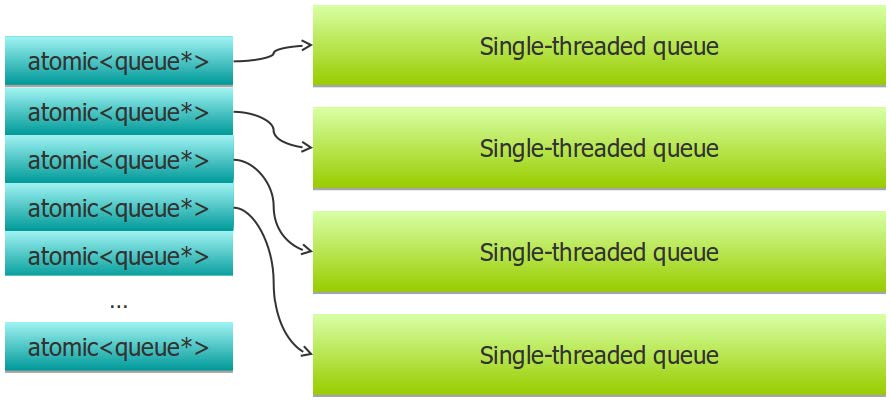
\includegraphics[width=0.7\textwidth]{content/2/chapter7/images/22.jpg}\\
圖7.22 - 基於通過原子指針訪問數組子隊列的非順序一致隊列
\end{center}

需要訪問隊列的線程必須獲得一個子隊列,可以從指針數組的任何元素開始。如果為空,則該子隊列當前處於繁忙狀態,然後嘗試下一個元素,以此類推,直到只剩下一個子隊列。此時,只有一個線程在子隊列上操作,因此不需要線程安全(子隊列甚至可以是\texttt{std::queue})。操作(\texttt{push}或\texttt{pop})完成後,線程原子性地將子隊列指針寫回數組,將子隊列的所有權返回給隊列。

\texttt{push}操作必須繼續嘗試剩下的子隊列,直到找到子隊列為止(或者,可以允許\texttt{push}在嘗試一定次數後失敗,向調用者發出隊列太忙的信號)。\texttt{pop}操作可能會保留一個子隊列,結果發現是空的。這種情況下,必須嘗試從另一個子隊列中彈出(可以在隊列中保持元素的原子計數,若隊列是空的,可以快速返回)。

當然,\texttt{pop}可能在一個線程上失敗,並報告隊列為空。實際上,這並不是因為另一個線程將新數據推入隊列。但這可能發生在併發隊列上,一個線程檢查隊列大小,發現隊列是空的,但在控制權返回給調用者之前,隊列可能會成為非空隊列。同樣,順序一致性對多個線程的可見性不一致性,需要進行了一些限制,而非順序一致性隊列使彈出元素的順序變得不確定。儘管順序有些亂,但還能接受。

不過,這並不是適用於所有數據結構,當大多數類似於隊列順序可以接受時,順序不一致可以產生明顯的性能提升,特別是在有許多線程的系統中。在一個運行許多線程的大型x86服務器上,進行順序不一致隊列擴展後的情況:

%\hspace*{\fill} \\ %插入空行
\noindent
\textbf{03b\_noncst\_queue.C}
\begin{center}
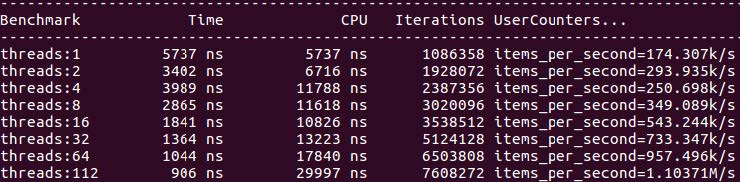
\includegraphics[width=0.9\textwidth]{content/2/chapter7/images/23.jpg}\\
圖7.23 - 順序不一致隊列的性能
\end{center}

這個基準測試中,所有線程都執行\texttt{push}和\texttt{pop}操作,並且元素相當大(複製每個元素需要複製1KB的數據)。為了進行比較,自旋鎖保護的\texttt{std::queue}在單個線程上具有相同的性能(大約每秒170k個元素),但根本沒有擴展性(整個操作都是鎖定的),而且性能下降得很慢(由於鎖定的開銷),對於最大線程數來說,性能會下降到(大約)每秒130k個元素。

當然,若出於性能考慮,可以接受順序不一致程序的混亂,那麼許多其他數據結構也可以使用這種方法。

當涉及到併發順序容器(如堆棧和隊列)時,我們要討論的最後一個主題是如何處理需要更多內存的情況

\subsubsubsection{7.4.3\hspace{0.2cm}並行數據結構的內存管理}

現在來討論內存管理的問題,之前假設數據結構的初始內存分配已經足夠,至少對於不會使整個操作變成單線程的無鎖數據結構來說是這樣的。本章中看到鎖保護的和順序不一致的數據結構沒有這個問題,在鎖或搶佔所有權的方式下,只有一個線程操作特定的數據結構,所以內存按照常規的方式分配。

對於無鎖數據結構,內存分配是一個重大挑戰。這通常是一個耗時的操作,特別是當數據必須複製到新位置時。多個線程可能會讓數據結構的內存耗盡,通常只有一個線程可以添加新的內存(很難讓那部分也變成多線程),其餘的線程必須等待。對於這個問題沒有較好的通用解決方案,這裡只是給出一些建議。

首先,最好的選擇是避免這個問題。當需要無鎖數據結構時,可以估計其最大容量並預分配內存,例如:知道要進入隊列的數據元素的總數。或者可以將問題推給調用者,可以告訴調用者數據結構的容量不足,而不是增加內存。對於無鎖數據結構的性能來說,這可能是一個可以接受的折衷方案。

如果需要增加內存,最理想的做法是添加內存時,但不復制現有數據結構。這意味著不能簡單地分配更多內存,並將所有內容複製到新位置。相反,必須將數據存儲在固定大小的內存塊中,就像\texttt{std::deque}一樣。當需要更多內存時,會分配另一個內存塊,通常會有一些指針地址需要更改,但不會複製數據。

完成內存分配的所有情況下,這是很少發生的事件。如果不是這樣,那麼使用由鎖或獨佔所有權保護的單線程的數據結構就好。這個罕見事件的性能不是關鍵,可以簡單地鎖定整個數據結構,並讓一個線程執行內存分配和必要的更新。關鍵的是公共內存地址,也就是意味著不需要更多內存的地址,所以程序會運行的很快。

這個想法非常簡單,不希望每次都在每個線程上獲取內存鎖,串行化整個程序。也不需要這樣做,大多數時候,不會內存不足,也不需要這個鎖。因此,需要檢查原子標誌。只有當內存分配正在進行,並且所有線程都必須等待時,才會設置該標誌:

\begin{lstlisting}[style=styleCXX]
std::atomic<int> wait; // 1 if managing memory
if (wait == 1) {
	… wait for memory allocation to complete …
}
if ( … out of memory … ) {
	wait = 1;
	… allocate more memory …
	wait = 0;
}
… do the operation normally … 
\end{lstlisting}

這裡的問題是,多個線程可能會在設置等待標誌之前同時檢測內存不足的情況。然後,嘗試向數據結構中添加更多的內存,這通常會導致競爭(重新分配底層內存很少是線程安全的)。不過,有一種簡單的解決方案,稱為\textbf{雙重檢查鎖},它同時使用互斥鎖(或另一個鎖)和原子標誌。如果標誌沒有設置,那麼一切正常,可以照常進行。如果設置標誌,則必須獲取鎖,並再次檢查該標誌:

\begin{lstlisting}[style=styleCXX]
std::atomic<int> wait;  // 1 if managing memory
std::mutex lock;
while (wait == 1) {};  // Memory allocation in progress
if ( … out of memory … ) {
	std::lock_guard g(lock);
	if (… out of memory …) { // We got here first!
		wait = 1;
		… allocate more memory …
		wait = 0;
	}
}
… do the operation normally …
\end{lstlisting}

第一次,檢查內存不足的情況,沒有任何鎖。速度很快,大多數時候,不會遇到內存不足。第二次,在鎖下檢查它,在鎖下可以保證一次只有一個線程在執行。多線程可能會檢測到內存不足,但第一個獲得鎖的線程是處理這種情況的線程,所有剩餘的線程都在等待鎖。當它們獲得鎖時,則進行第二次檢查(因此,雙重檢查鎖),發現內存充足。

這種方法可以泛化來處理罕見的特殊情況,但與其他代碼相比,以無鎖的方式實現這種情況要困難得多。某些情況下,甚至可能對空隊列的情況非常有用。如果兩個線程組不相互交互,那麼多個生產者或多個消費者的處理將需要原子遞增的索引。如果在特定的應用程序中,就能夠保證隊列很少(如果有的話)變成空,那麼可以選擇對於非空隊列來說非常快(無需等待)的實現,但如果隊列可能為空,則需要使用全局鎖。

好了,我們已經詳細地介紹了順序數據結構,接下來來研究一下節點數據結構。






























